\documentclass{article}

\usepackage[utf8]{inputenc}
\usepackage[T1]{fontenc}
\usepackage[francais]{babel}
\usepackage{xcolor}
\usepackage{listings}
\usepackage{mathptmx}
\usepackage{anyfontsize}
\usepackage{t1enc}
\usepackage[top=2cm, bottom=2cm, left=2cm, right=2cm]{geometry}
\usepackage{titlesec}
\usepackage{tikzducks}
\usepackage{titling}
\usepackage{graphicx}
\usepackage{wrapfig}
\usepackage{csquotes}
\usepackage[colorlinks = true,
            linkcolor = black,
            urlcolor  = black,
            citecolor = black,
            anchorcolor = black]{hyperref}
\usepackage[justification=centering]{caption}

\newcommand{\changeurlcolor}[1]{\hypersetup{urlcolor=#1}}

\renewcommand\maketitlehooka{\null\mbox{}\vfill}
\renewcommand\maketitlehookd{\vfill\null}

\definecolor{codegreen}{rgb}{0,0.6,0}
\definecolor{codegray}{rgb}{0.5,0.5,0.5}
\definecolor{codepurple}{rgb}{0.58,0,0.82}
\definecolor{backcolour}{rgb}{0.95,0.95,0.92}
\definecolor{codekeywords}{rgb}{0.1,0.53,0.92}

\lstdefinestyle{c++}{
    backgroundcolor=\color{backcolour},   
    commentstyle=\color{codegreen},
    keywordstyle=\color{codekeywords},
    numberstyle=\tiny\color{codegray},
    stringstyle=\color{codepurple},
    basicstyle=\ttfamily\footnotesize,
    breakatwhitespace=false,         
    breaklines=true,                 
    captionpos=b,                    
    keepspaces=true,                 
    numbers=left,                    
    numbersep=5pt,                  
    showspaces=false,                
    showstringspaces=false,
    showtabs=false,                  
    tabsize=2,
    texcl=false,
    inputencoding=utf8x,
    extendedchars=true,
    literate=
  {á}{{\'a}}1 {é}{{\'e}}1 {í}{{\'i}}1 {ó}{{\'o}}1 {ú}{{\'u}}1
  {Á}{{\'A}}1 {É}{{\'E}}1 {Í}{{\'I}}1 {Ó}{{\'O}}1 {Ú}{{\'U}}1
  {à}{{\`a}}1 {è}{{\`e}}1 {ì}{{\`i}}1 {ò}{{\`o}}1 {ù}{{\`u}}1
  {À}{{\`A}}1 {È}{{\'E}}1 {Ì}{{\`I}}1 {Ò}{{\`O}}1 {Ù}{{\`U}}1
  {ä}{{\"a}}1 {ë}{{\"e}}1 {ï}{{\"i}}1 {ö}{{\"o}}1 {ü}{{\"u}}1
  {Ä}{{\"A}}1 {Ë}{{\"E}}1 {Ï}{{\"I}}1 {Ö}{{\"O}}1 {Ü}{{\"U}}1
  {â}{{\^a}}1 {ê}{{\^e}}1 {î}{{\^i}}1 {ô}{{\^o}}1 {û}{{\^u}}1
  {Â}{{\^A}}1 {Ê}{{\^E}}1 {Î}{{\^I}}1 {Ô}{{\^O}}1 {Û}{{\^U}}1
  {œ}{{\oe}}1 {Œ}{{\OE}}1 {æ}{{\ae}}1 {Æ}{{\AE}}1 {ß}{{\ss}}1
  {ç}{{\c c}}1 {Ç}{{\c C}}1 {ø}{{\o}}1 {å}{{\r a}}1 {Å}{{\r A}}1
  {€}{{\EUR}}1 {£}{{\pounds}}1
}
\lstset{style=c++}


\title{Ouai}
\author{Arquillière Mathieu - Zangla Jérémy}
\date{\today}

% \begin{lstlisting}[style=c++]
% \end{lstlisting}
% \changeurlcolor{blue}\href{run:../Documentation/latex/refman.pdf}{Lien vers la documentation Doxygen}

\begin{document}

\begin{titlepage}
  \maketitle
\end{titlepage}

\tableofcontents
\listoffigures
\newpage

\section{Prise en main de l'application}
\subsection{Organisation de l'application}
\begin{wrapfigure}[20]{r}[0pt]{0.3\textwidth}
  \vspace{-50pt}
  \label{Menu de navigation}
  \centering
  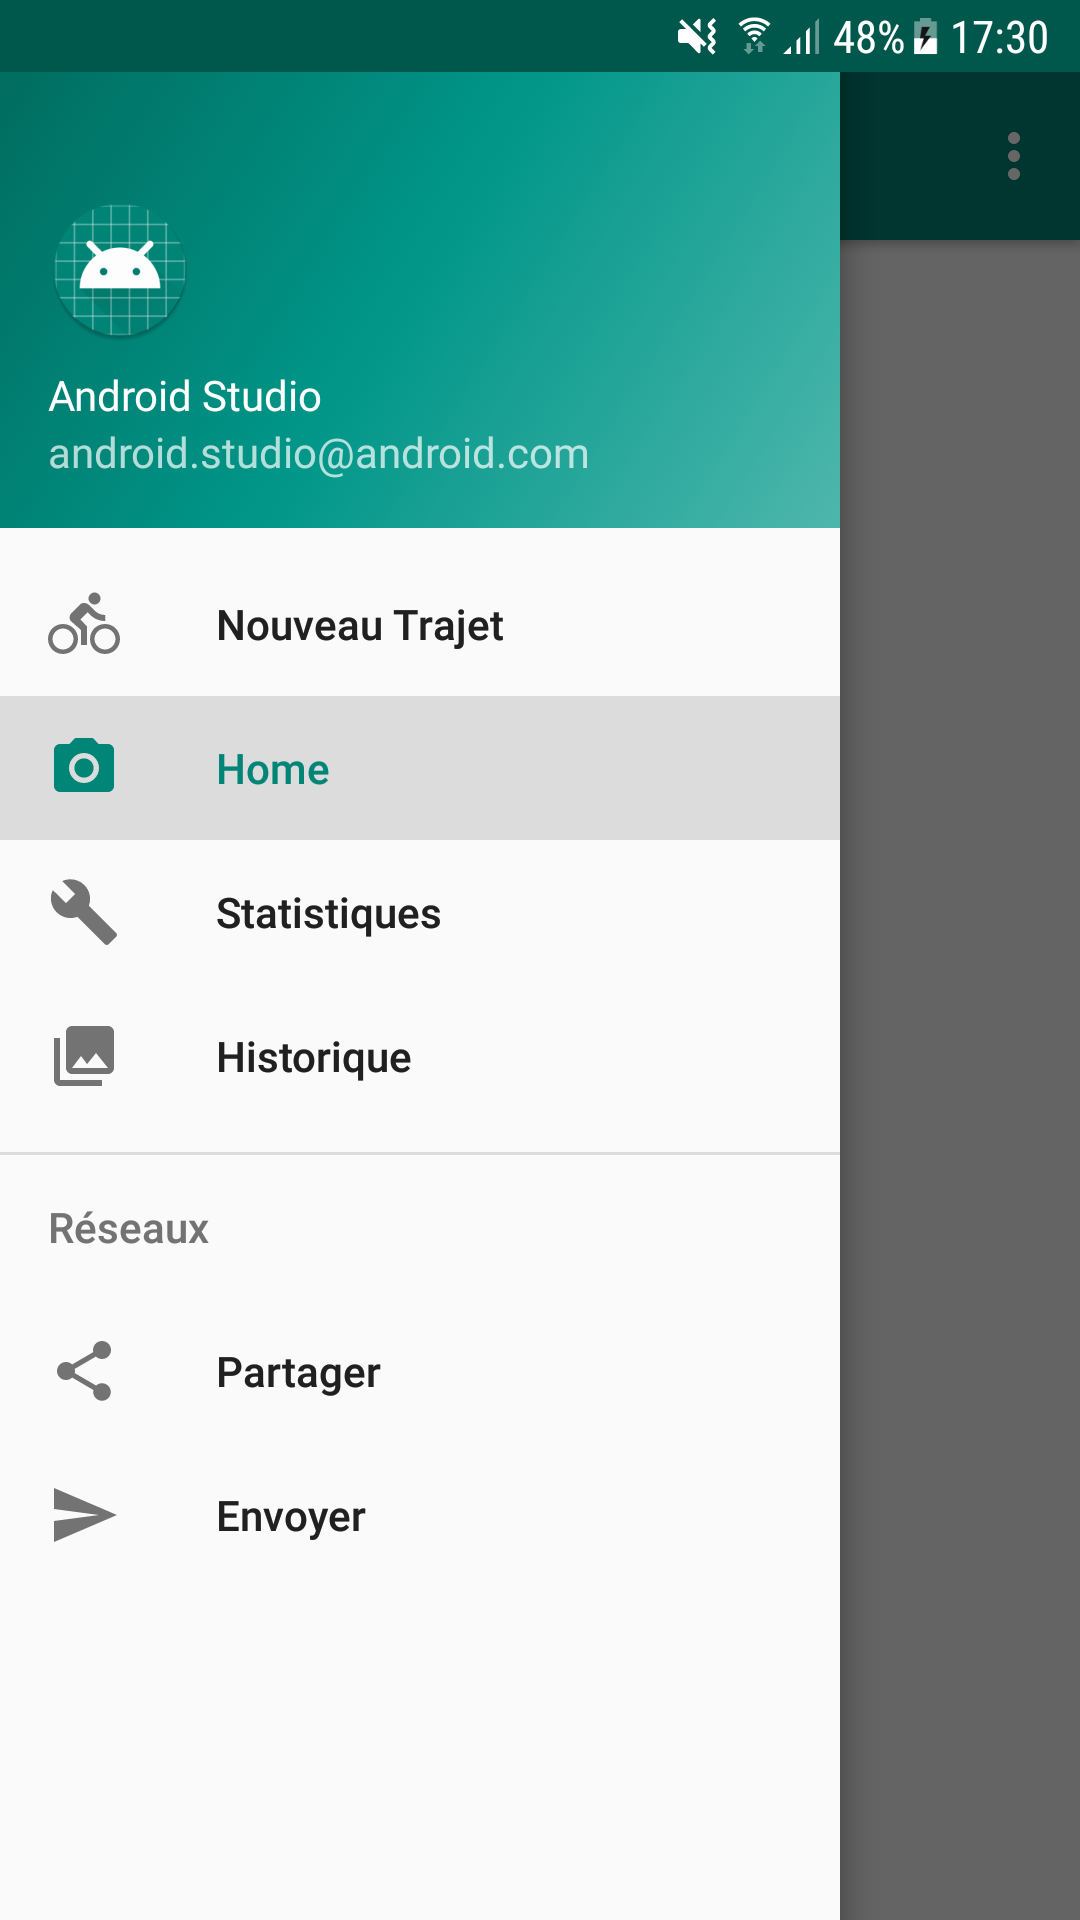
\includegraphics[scale=0.13]{images/navigation-menu.png}
  \caption{Capture d'écran du menu de navigation}
\end{wrapfigure}
L'application se rapproche beaucoup d'une application android standard. Elle possède une page d'accueil vide à notre stade de développement mais
elle est censée contenir à terme les derniers trajets effectués et partagés par nos amis dans l'application.

Un menu de navigation est accessible depuis le bouton en haut à gauche de l'écran ou en faisant glisser le doigt de gauche à droite de l'écran.
Ce menu permet d'accéder aux différentes fonctionnalités de logiciel. Ce menu devait également afficher notre nom d'utilisateur et
possiblement un icône pour nous représenter.

Les onglets effectifs sont les onglets "Nouveau Trajet" et "Historique". Les autres n'ont pas pu être développés.


% \begin{figure}
%   \label{Menu de navigation}
%   \centering
%   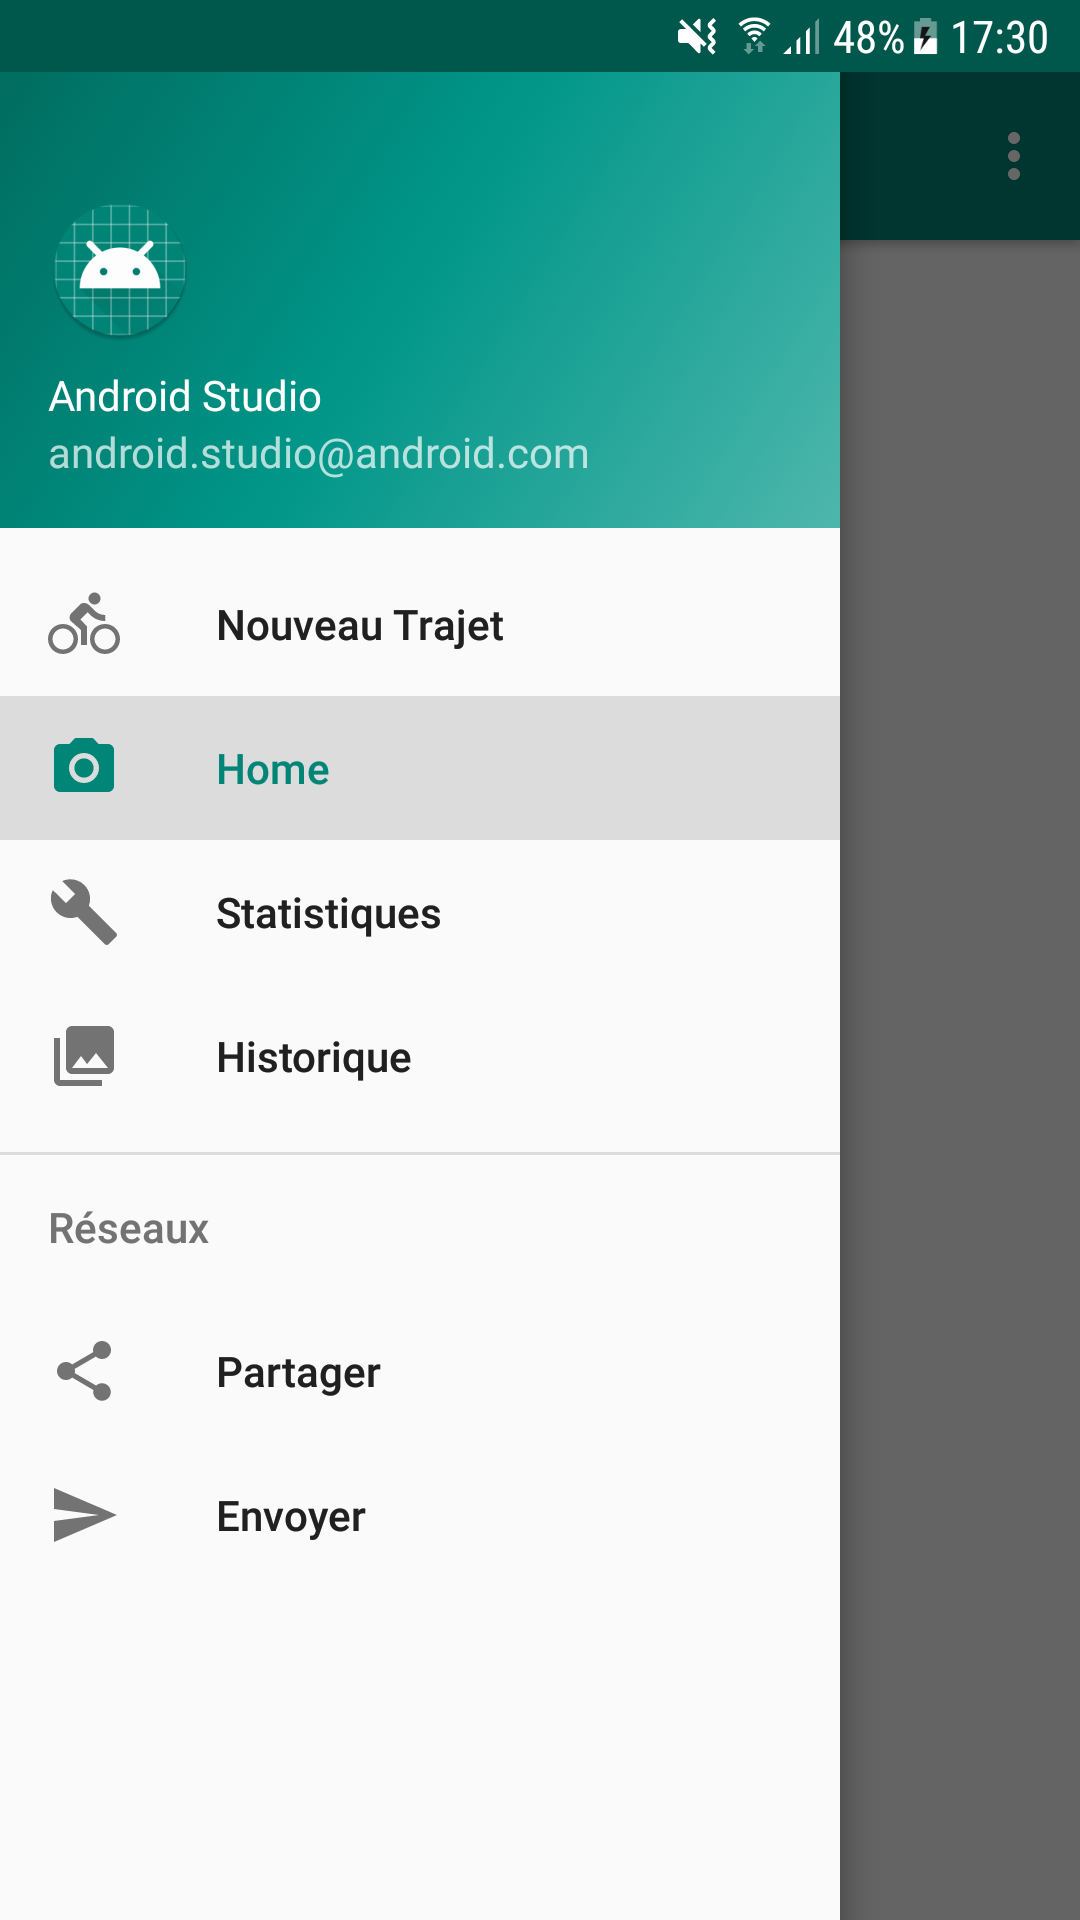
\includegraphics[scale=0.13]{images/navigation-menu.png}
%   \caption{Capture d'écran du menu de navigation}
% \end{figure}

\subsection{Onglet "Nouveau Trajet"}
Cet onglet est la partie principale de l'application. Il contient une carte dynamique (google map) et un bouton. Lorsqu'on clique sur ce
bouton, on lance alors la création d'un nouveau trajet. Cela se remarque grâce au bouton qui a changé de texte et de fonction, il permet
alors d'indiquer la fin du trajet, et de la carte qui affiche maintenant un point nous représentant sur la carte. Dès lors, lorsqu'on bouge
le gps le détecte et transmet un nouveau point à la carte. Notre position change donc et la suite de ces points affiche un chemin visible
sur la carte.

Une fois le trajet voulu réalisé, on clique sur le bouton en bas de l'écran pour le terminer. Ceci a pour effet de faire apparaître une
petite fenêtre en superposition de la carte. Ce "pop-up" contient une zone de texte et un bouton et nous permet de rentrer un nom pour
le trajet que l'on vient d'effectuer. Une fois ce nom rentré, le trajet s'enregistre sur le téléphone et on peut de nouveau créer un
autre trajet.
\begin{figure}[ht]
  \label{Nouveau trajet}
  \centering
  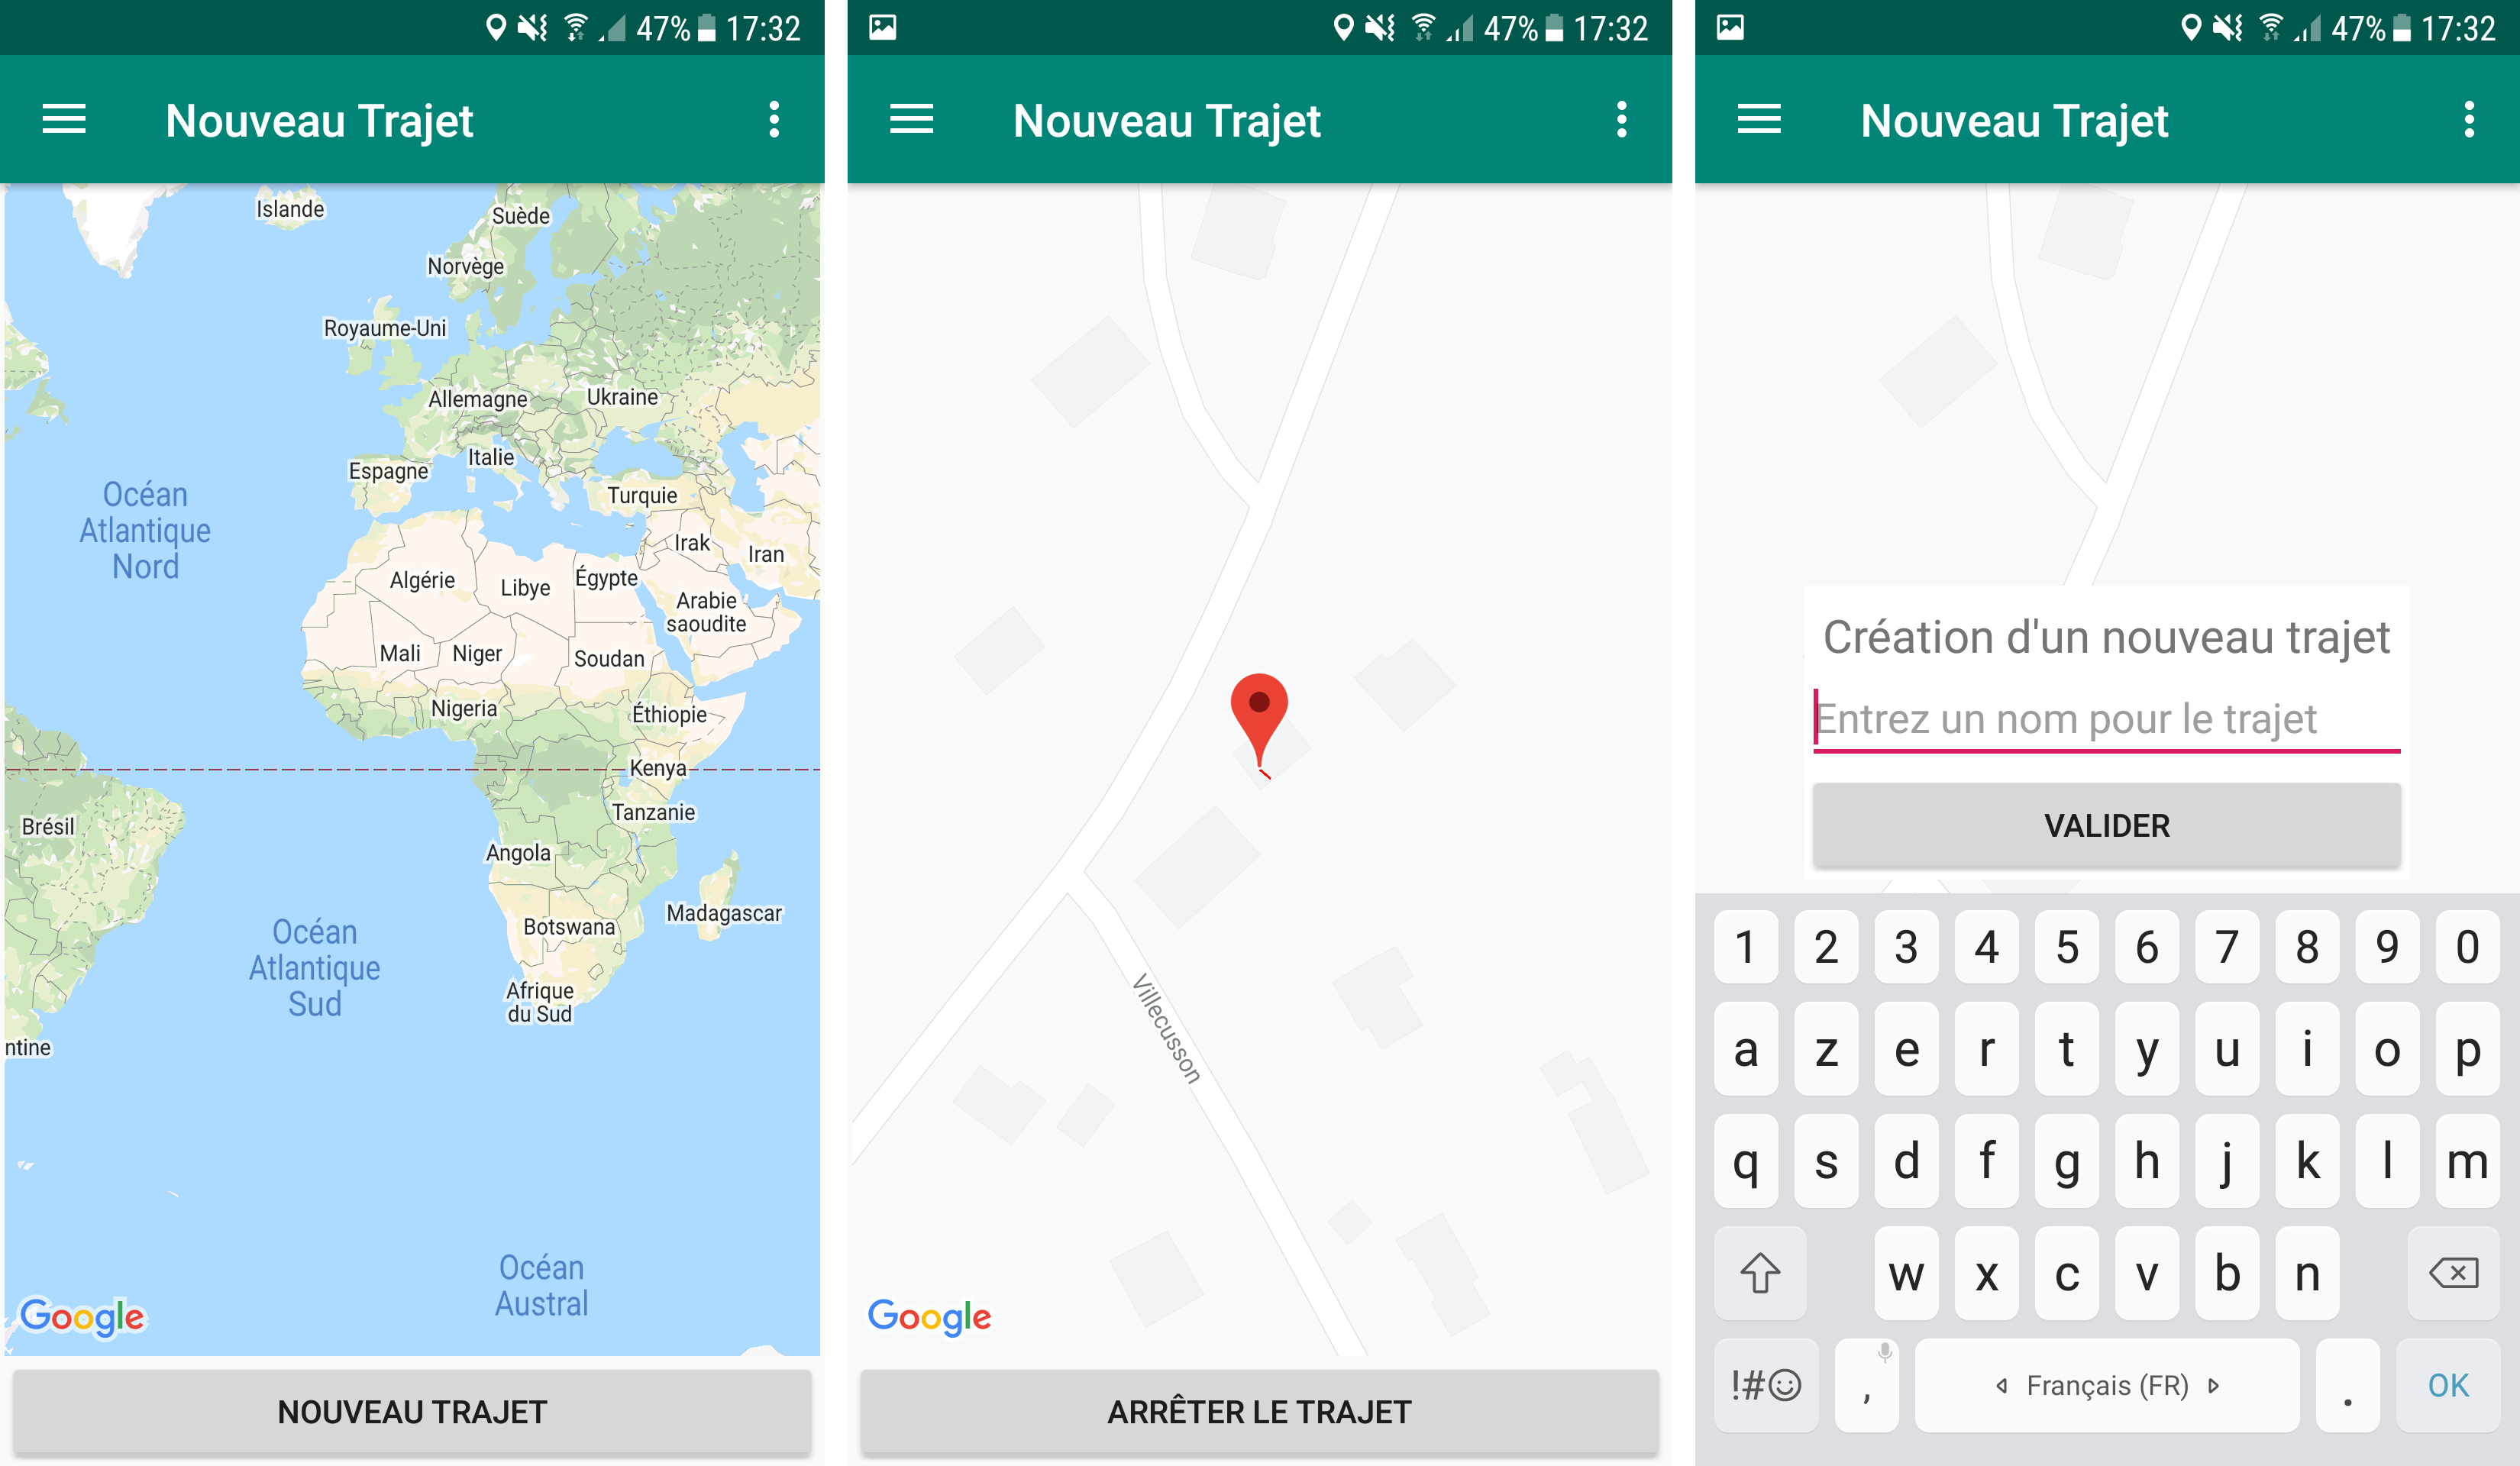
\includegraphics[scale=0.14]{images/nouveau-trajet.png}
  \caption{Multiples captures d'écrans lors d'un nouveau trajet}
\end{figure}

\subsection{Onglet "Historique"}
Cet onglet contient l'ensemble des trajets effectués et enregistrés. Ils s'affichent du plus récent au plus vieux. Chaque trajet est représenté
par une "card", un conteneur composé du nom du trajet, de sa date de création, de sa durée et d'une capture d'écran de la carte prise au moment
de sa création. Si il y a trop de trajets et qu'ils ne rentrent pas tous dans l'écran, on peut les faire défiler grâce à une barre de défilement
en faisant glisser son doigt de bas en haut. Chaque "card" est cliquable et amène vers une page dédié au trajet.
\begin{figure}[ht]
  \label{Historique}
  \centering
  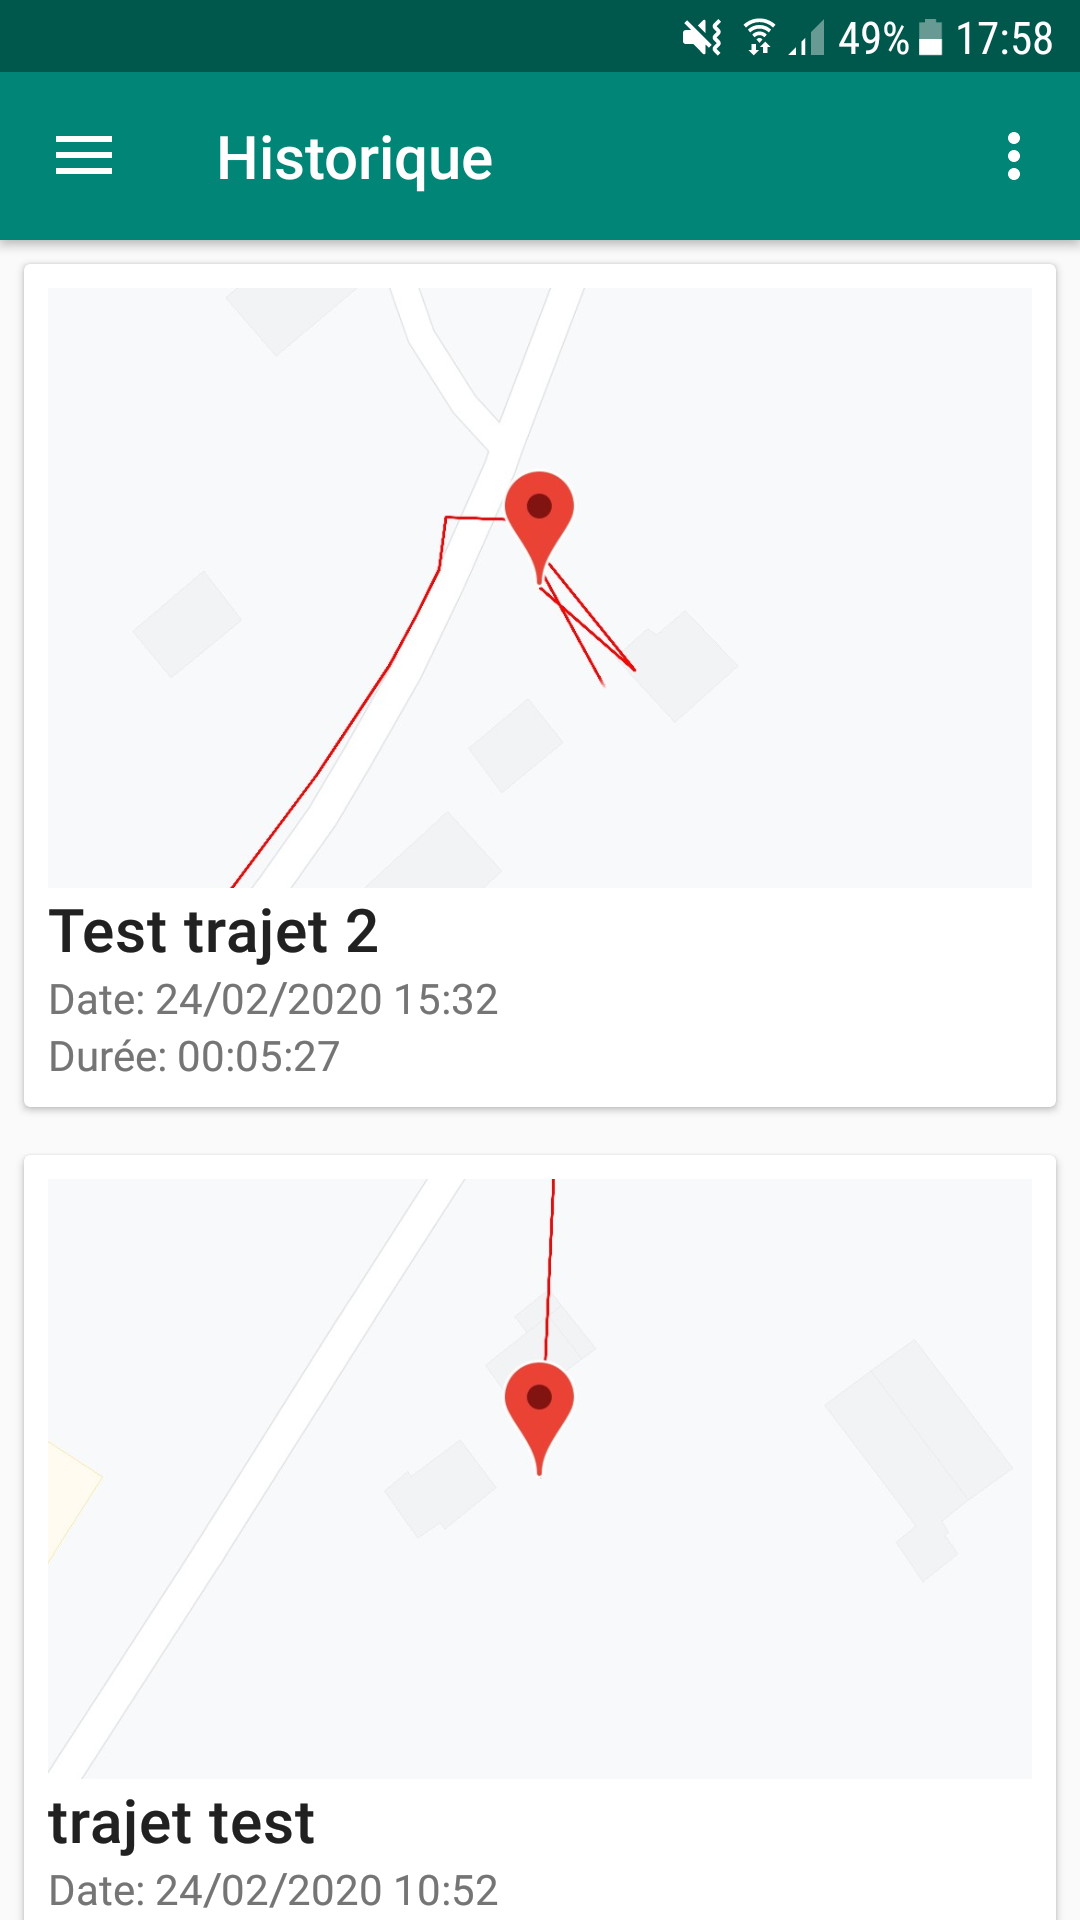
\includegraphics[scale=0.13]{images/historique.png}
  \caption{Capture d'écran de l'historique}
\end{figure}

\subsection{Page "Trajet"}
\begin{wrapfigure}[5]{r}[0pt]{0.5\textwidth}
  \label{Trajet}
  \centering
  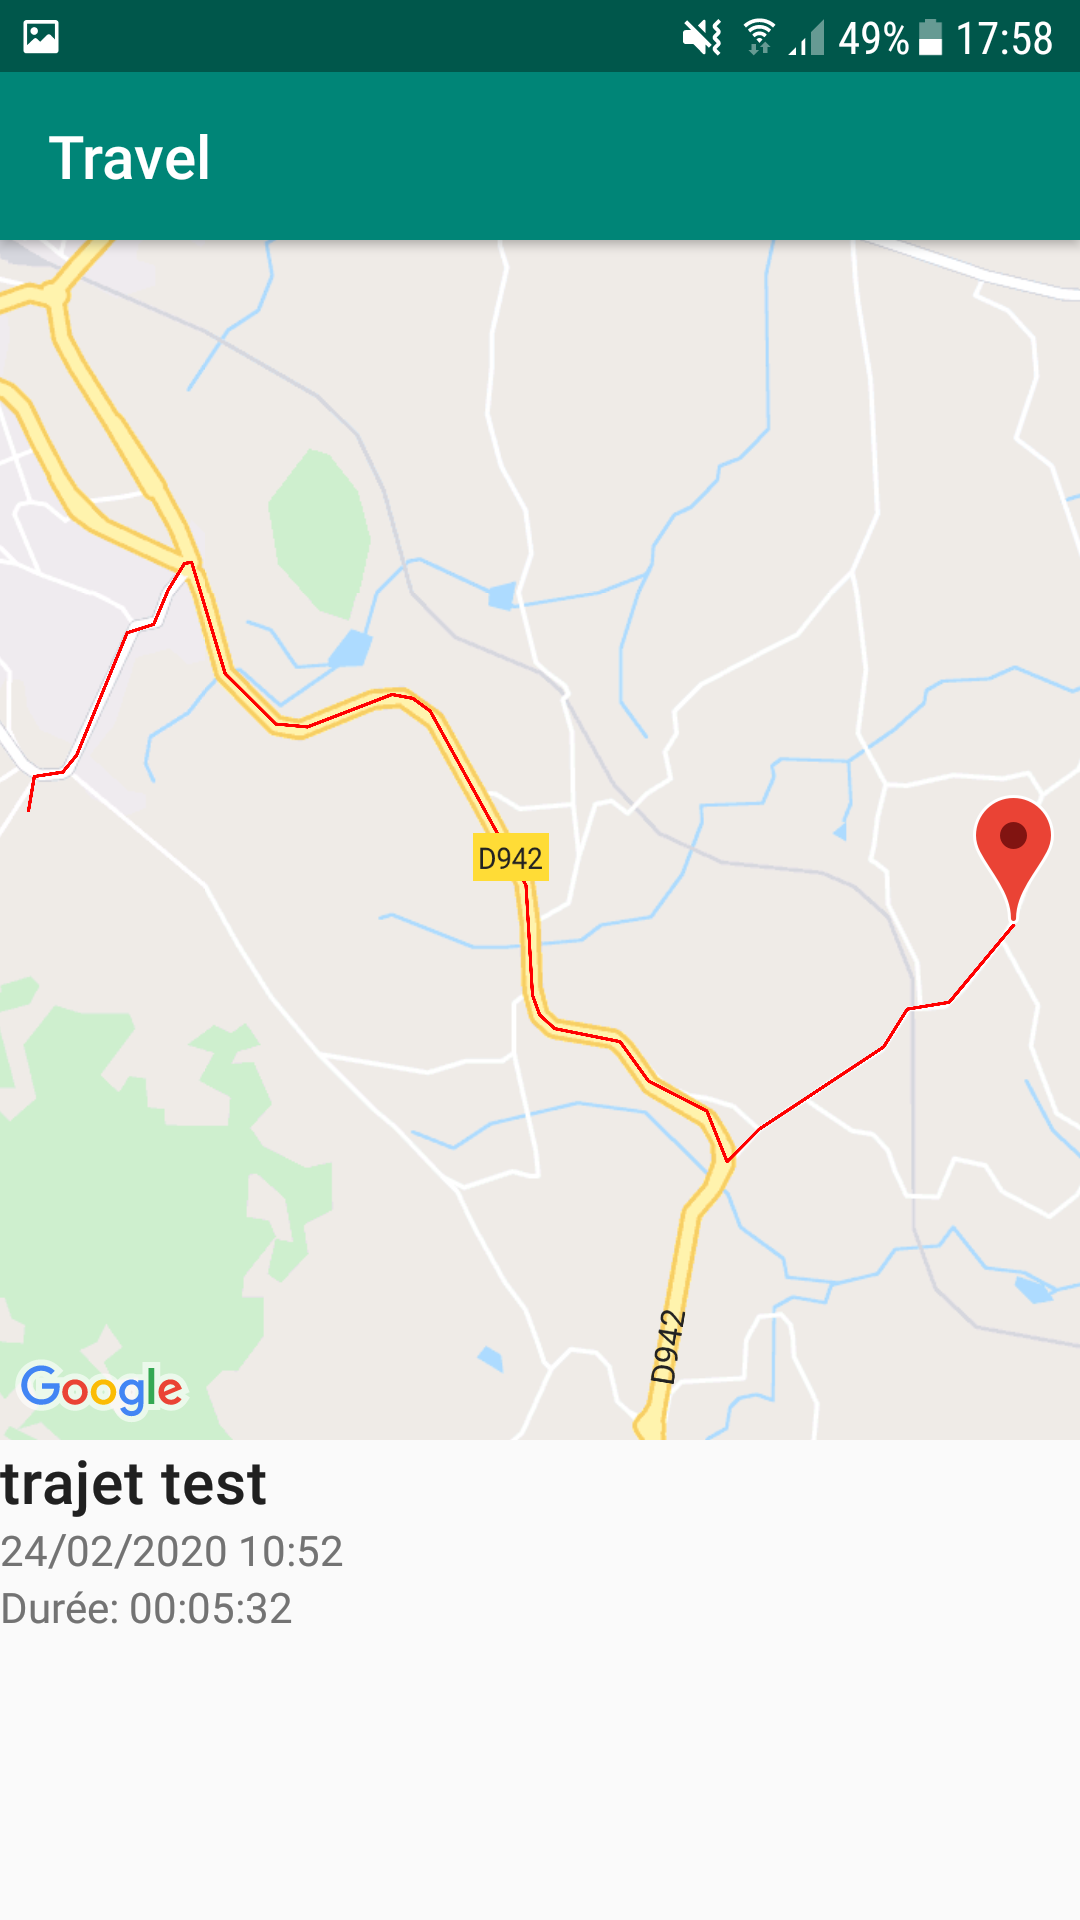
\includegraphics[scale=0.13]{images/travel.png}
  \caption{Capture d'écran d'une page d'un traje}
\end{wrapfigure}
Une page de trajet s'affiche lorsqu'on clique sur l'un dans l'historique. Cette page détaille le trajet avec son nom, sa date de création et
sa durée mais créer aussi une nouvelle carte (google map) sur laquelle est retracée le chemin effectué lors de la création du trajet.

% \begin{figure}[ht]
%   \label{Trajet}
%   \centering
%   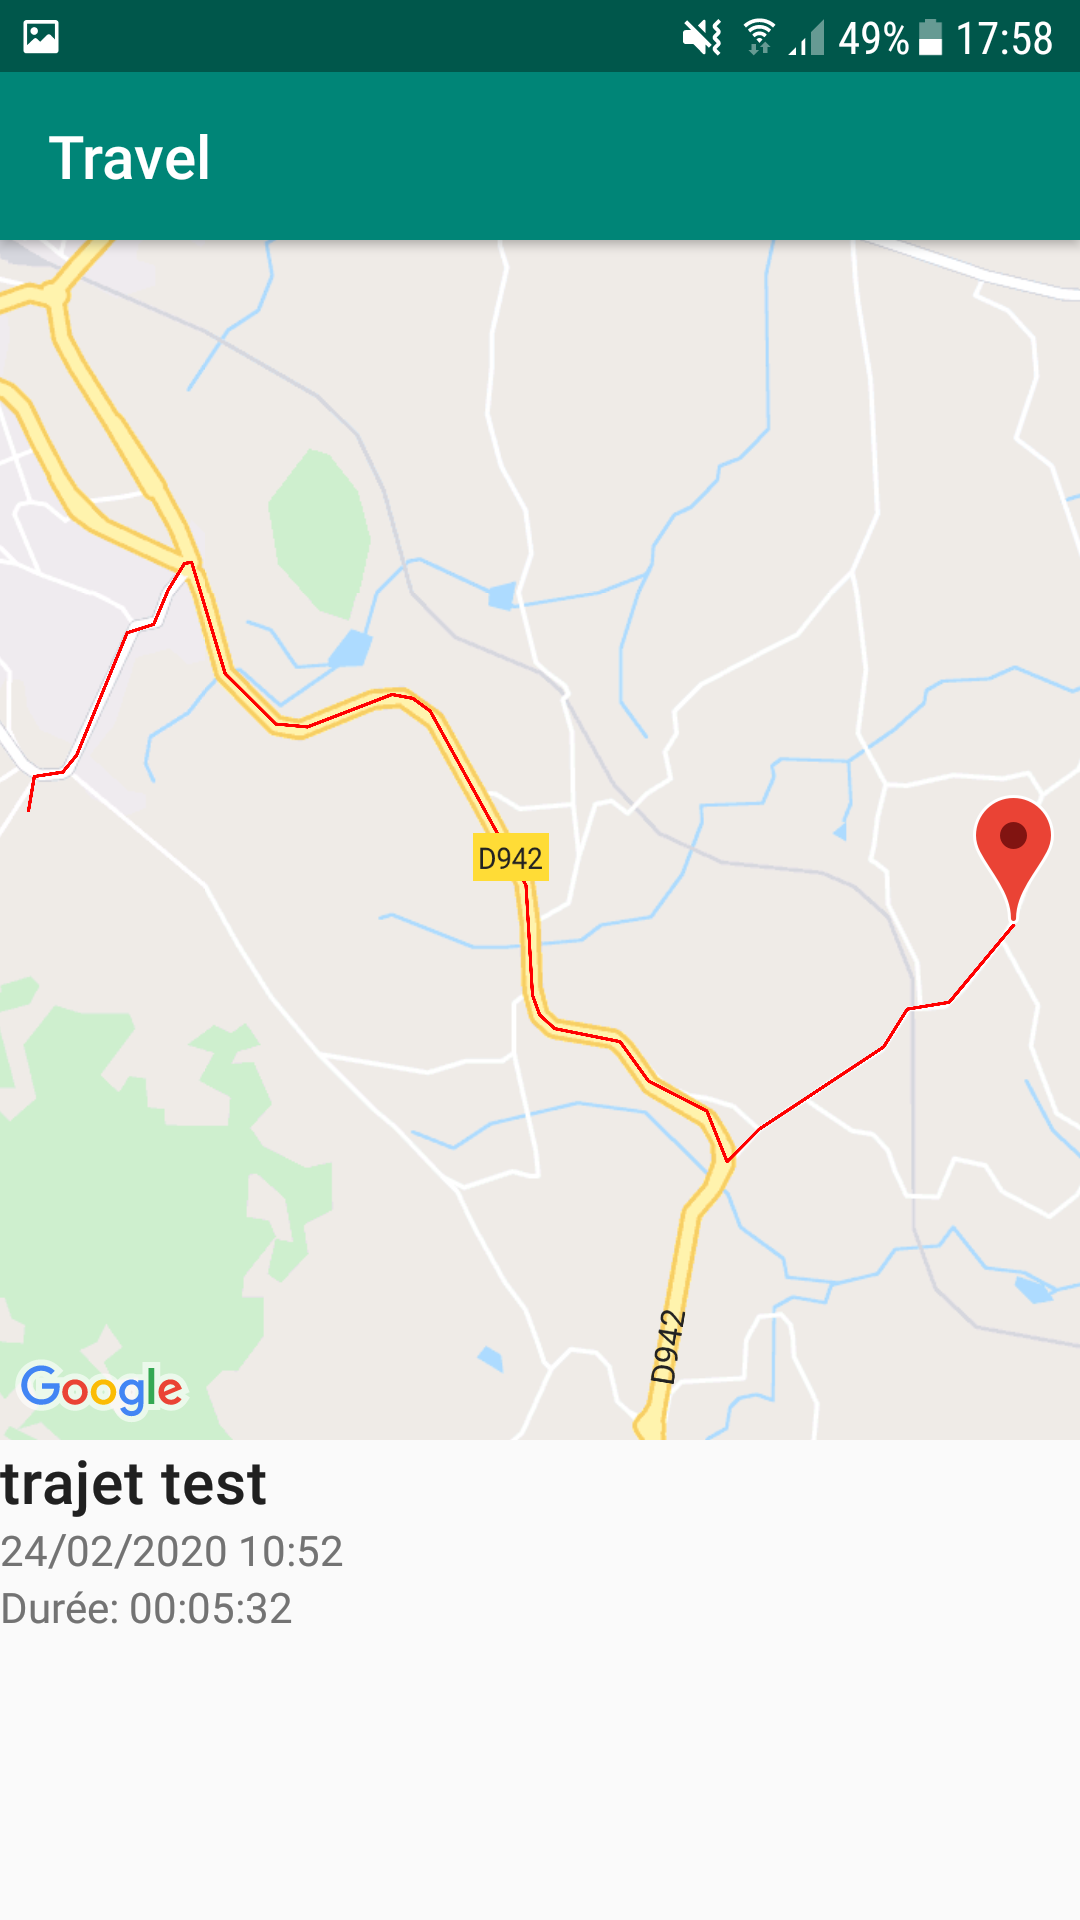
\includegraphics[scale=0.13]{images/travel.png}
%   \caption{Capture d'écran d'une page d'un trajet}
% \end{figure}

\newpage
\section{Analyse du problème}
\subsection{Le problème}
La problèmatique de ce projet est comment aider un cycliste à réaliser des trajets qui ne sont pas répertoriés sur des cartes. L'idée est qu'un cycliste, 
en particulier ceux qui pratiquent le vélo tout terrain, n'a pas à sa disposition des cartes précises des chemins possibles. En effet,
lorsqu'on s'éloigne des routes pour utiliser des chemins (à travers des forêts par exemple) les cartes papiers ou électroniques ne sont pas
très exhaustives. La solution serait donc de fournir un outil permettant aux cyclistes de réaliser leur propres trajets dans ces
chemins et de pouvoir les partager à d'autres cyclistes qui souhaiteraient effectuer ces trajets.

\subsection{Proposition d'une solution}
L'outil qui permetterait de résoudre ce problème serait donc utilisable par un cycliste afin de sauvegarder son trajet. La solution la plus évidente
est d'utiliser un smartphone, qui possède un GPS, une interface et une connexion internet. La réponse au problème serait donc une application
smartphone.

\subsubsection{Fonctionnalités principales}
\begin{enumerate}
  \item L'objectif principal est de capturer via un GPS les coordonnées du trajet effectué par l'utilisateur afin de tracer celui-ci sur une carte
  électronique.
  \item Il faut également pouvoir sauvegarder ce trajet pour que l'on puisse le consulter ultérieurement et s'en servir pour refaire le trajet.
  Dans l'idéal cette fonctionnalité ressemblera au fonctionnement d'un GPS classique indiquant à la fois notre position et notre progression dans le tracé.
  \item Enfin, les trajets pourront être partagés et utilisés par d'autres utilisateurs de l'application.
\end{enumerate}

\subsubsection{Fonctionnalités bonus}
\begin{enumerate}
  \item Les trajets faits ne sont pas forcément ce qu'on aurait voulu tracer et sauvegarder dans l'application. Une solution pourrait être de
  rendre possible la modification d'un trajet afin de le re-dessiner.
  \item Pour rendre l'application plus attractive et moins limité aux amateur de cyclisme, elle pourrait adopter le comportement d'un réseau
  social, avec plus d'interaction entre les utilisateurs (fil d'actualité, messages privés) et plus de sport utilisant ce principe (course à pied, moto).
\end{enumerate}


\section{Organisation}
\subsection{Arborescence}

\newpage
\appendix
\section{Manuel d'utilisation}

\end{document}